\section{Evaluation and Error Calculation}
\label{sec:Evaluation}
% --------------
% Speed of Sound
% --------------
\subsection{Speed of Sound}
\label{subsec:Speed_of_Sound}
To determine the speed of sound, the propagation time of a sound pulse over the distance $s=(2.561\pm0.003)\ m$ was measured 20 times (see table \ref{tab:Speed_of_Sound_Measurements}). The ambient temperature was $\vartheta=23$ °C.

To calculate the speed of sound from the measured values, one has to calculate the mean value of the duration $t_i$ and its error. To do this in Excel, the function "AVERAGE()" is used to calculate the mean value. This function implements equation \ref{eq:Arithmetic_Mean}. To calculate the error of the mean value, the function "STDEV.S()" is used, which implements equation \ref{eq:Arithmetic_Mean_Error}. The same thing can be achieved using the software QtiPlot. The measured values are shown in the following figure \ref{fig:Sound_Propagation_Time}:
\begin{figure}[H]
	\centering
	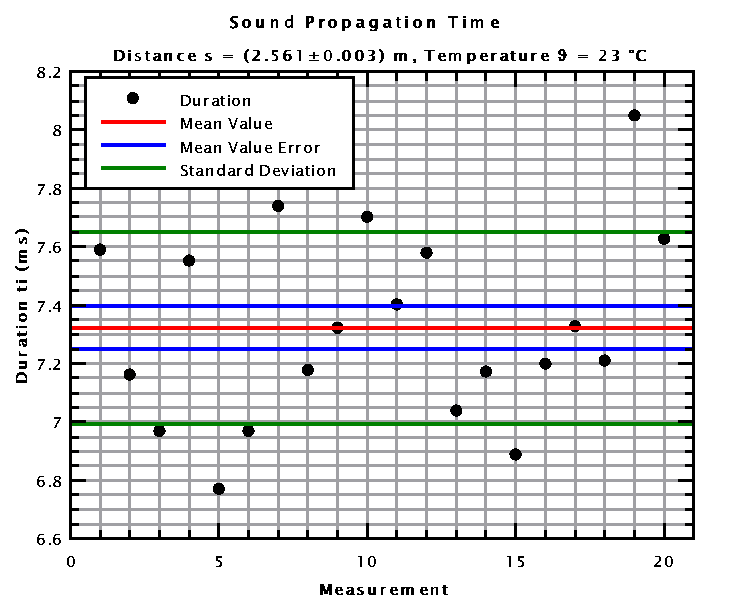
\includegraphics[scale=1]{Sound_Propagation_Time}
	\caption{Sound Propagation Time}
	\label{fig:Sound_Propagation_Time}
\end{figure}
Equation \ref{eq:Experimental_Standard_Deviation} is used to calculate the experimental standard deviation. This can be done by using the Excel function "STDEV.S()" again. If the equation \ref{eq:Arithmetic_Mean} for the mean value error is compared to the equation \ref{eq:Experimental_Standard_Deviation} for the experimental standard deviation, it becomes apparent that only an $\sqrt{n}$ is missing in the denominator. This can easily be fixed by dividing the function by $\sqrt{n}$. QtiPlot allows for direct calculation of the experimental standard deviation for an entire column of values.
\newpage
The comparison between Excel and QtiPlot is shown in the following table \ref{tab:Comparison_Speed_of_Sound_Measurements}:
\begin{table}[H]
	\centering
	\renewcommand{\arraystretch}{1.2}
	\begin{tabular}{c c c c}
		\hline
		\textbf{Software} & \textbf{Mean Value $\overline t$} & \textbf{Mean Value Error $s_{\overline{t}}$} & \textbf{Standard Deviation $s$} \\
		\hline
		Excel & $7.3225\cdot10^{-3}$ s & $7.35308\cdot10^{-5}$ s & $3.28840\cdot10^{-4}$ s \\
		QtiPlot & $7.3225\cdot10^{-3}$ s & $7.35308\cdot10^{-5}$ s & $3.28840\cdot10^{-4}$ s \\ \hline
	\end{tabular}
	\caption{Comparison between the calculated values}
	\label{tab:Comparison_Speed_of_Sound_Measurements}
\end{table}
The following equation is used to calculate the mean value of the speed of sound:
\begin{equation}
\overline{v}=\frac{\overline s}{\overline t}=\frac{2.561\ m}{7.3225\cdot10^{-3}\ s}=349.744\ \frac{m}{s}
\label{eq:Speed_of_Sound}
\end{equation}
\\
Equation \ref{eq:Error_Propagation} is used to calculate the uncertainty:
\begin{equation}
s_{\overline{v}}=\sqrt{\left(\frac{\partial v}{\partial s}\Biggr|_{\overline v}\cdot s_{\overline{s}}\right)^2 + \left(\frac{\partial v}{\partial t}\Biggr|_{\overline v}\cdot s_{\overline{t}}\right)^2}=\sqrt{\left(\frac{1}{\overline t}\cdot s_{\overline{s}}\right)^2 + \left(-\frac{\overline{s}}{\overline{t}^2}\cdot s_{\overline{t}}\right)^2}=3.53586\ \frac{m}{s}
\end{equation}
\\
The derived speed of sound is as follows:
\begingroup
\Large
\begin{equation}
v=\overline{v}\pm s_{\overline v}=(350\pm4)\ \frac{m}{s}
\end{equation}
\endgroup
\newpage
% ------------
% Iron Content
% ------------
\subsection{Iron Content}
\label{subsec:Iron_Content}
The iron content in an alloy was determined by various methods. Therefore, the accuracy varies between the different measurements.

In Excel, the mean value and its error are calculated the same way as in section \ref{subsec:Speed_of_Sound}. The weighted mean value can be calculated by using the "SUMPRODUCT()" function. The formula is as follows:
\[
=\text{SUMPRODUCT}(\overline{x_1}:\overline{x_n};1/(s_{\overline{x1}}:s_{\overline{xn}})\textasciicircum 2)/\text{SUM}(s_{\overline{x1}}:s_{\overline{xn}})
\]
\\
The measured values (see table \ref{tab:Iron_Content_Measurements}) and their respective error are shown in figure \ref{fig:Iron_Content}. Furthermore, the weighted mean value was calculated by a weighted regression fit in QtiPlot (also shown in fig. \ref{fig:Iron_Content}).
\begin{figure}[H]
	\centering
	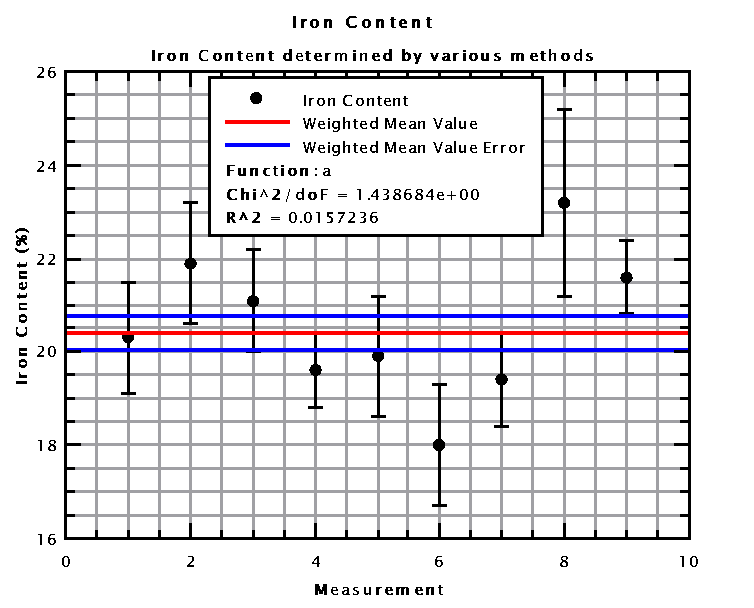
\includegraphics[scale=1]{Iron_Content}
	\caption{Iron Content}
	\label{fig:Iron_Content}
\end{figure}
The comparison for the mean value and its error:
\begin{table}[H]
	\centering
	\renewcommand{\arraystretch}{1.2}
	\begin{tabular}{c c c}
		\hline
		\textbf{Software} & \textbf{Mean Value} & \textbf{Mean Value Error} \\
		\hline
		Excel & $20.5556$ \% & $0.519912$ \% \\
		QtiPlot & $20.5556$ \% & $0.519912$ \% \\ \hline
	\end{tabular}
	\caption{Comparison between the calculated values (Mean Value)}
	\label{tab:Comparison_Iron_Content_Mean_Value}
\end{table}
\newpage
The comparison for the weighted mean value and its error:
\begin{table}[H]
	\centering
	\renewcommand{\arraystretch}{1.2}
	\begin{tabular}{c c c}
		\hline
		\textbf{Software} & \textbf{Weighted Mean Value} & \textbf{Weighted Mean Value Error} \\
		\hline
		Excel & $20.4007$ \% & $0.361055$ \% \\
		QtiPlot & $20.4007$ \% & $0.361055$ \% \\ \hline
	\end{tabular}
	\caption{Comparison between the calculated values (Weighted Mean Value)}
	\label{tab:Comparison_Iron_Content_Weighted_Mean_Value}
\end{table}
\newpage
% ---------------
% Spring Constant
% ---------------
\subsection{Spring Constant}
\label{subsec:Spring_Constant}
To determine the spring constant of a pretensioned steel spring from the measured values (see table \ref{tab:Spring_Constant_Measurements}) the following equation is used to create a linear regression fit:
\begin{equation}
F=k\cdot z+F_0
\end{equation}
The measured values and the linear regression fit are shown in the following figure \ref{fig:Spring_Constant}:
\begin{figure}[H]
	\centering
	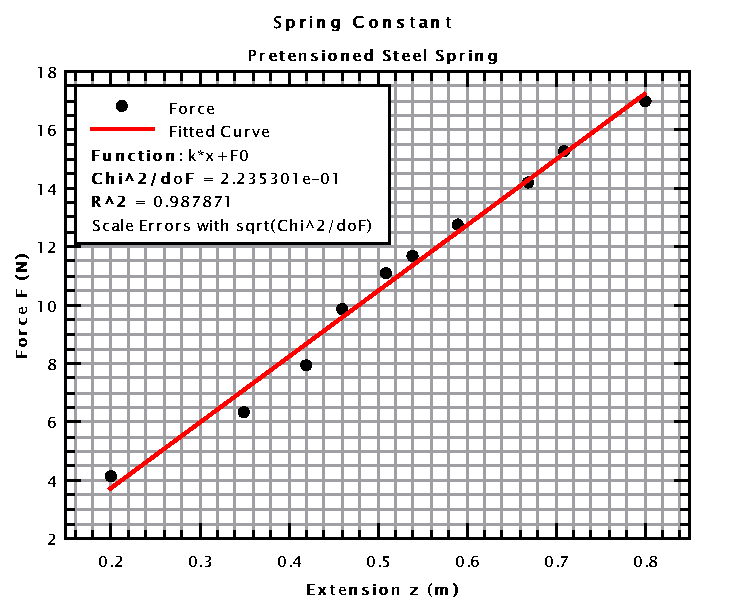
\includegraphics[scale=1]{Spring_Constant}
	\caption{Spring Constant}
	\label{fig:Spring_Constant}
\end{figure}
The values obtained from QtiPlot are shown in the following table \ref{tab:Calculated_Spring_Force_Parameters}:
\begin{table}[H]
	\centering
	\renewcommand{\arraystretch}{1.3}
	\begin{tabular}{c c}
		\hline
		\textbf{Spring Constant $k$} & \textbf{Pretension Force $F_0$} \\
		\hline
		$(22.5\pm0.9)\ \,^\text{N}\!/_\text{m}$ & $(-0.8\pm0.5)$\ N \\ \hline
	\end{tabular}
	\caption{Calculated Spring Force Parameters}
	\label{tab:Calculated_Spring_Force_Parameters}
\end{table}
The spring force can now be derived from the following equation:
\begin{equation}
F=22.5\ \,^\text{N}\!/_\text{m}\cdot z-0.8\ \text{N}
\end{equation}
\newpage
% --------
% Pendulum
% --------
\subsection{Pendulum}
\label{subsec:Pendulum}
The damped oscillation of a pendulum can be described by the following equation:
\begin{equation}
y=A\cdot \text{exp}(-\Gamma\cdot t)\cdot\text{sin}(2\cdot\pi\cdot f\cdot t-\delta)+y_0
\end{equation}
The values in table \ref{tab:Pendulum_Measurements} were measured with an ultrasonic sensor. The following figure \ref{fig:Pendulum} shows the measured distances as a function of time as well as the nonlinear fitted curve.
\begin{figure}[H]
	\centering
	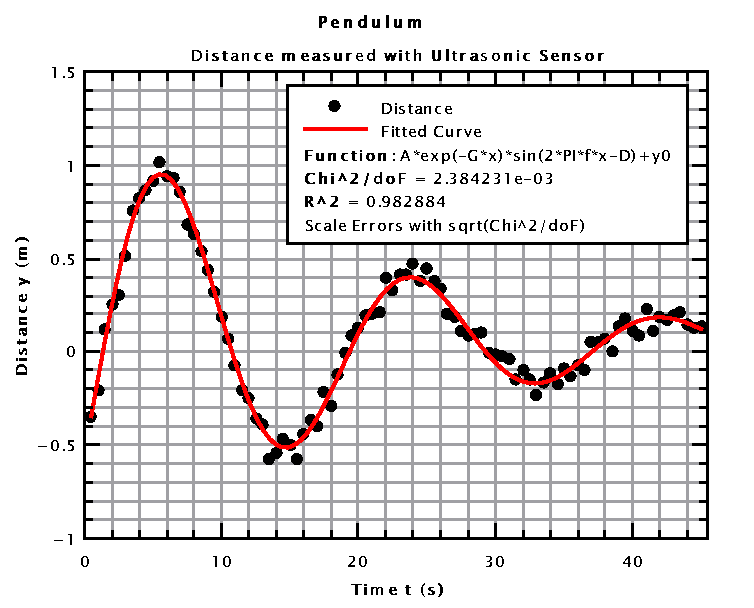
\includegraphics[scale=1]{Pendulum}
	\caption{Pendulum}
	\label{fig:Pendulum}
\end{figure}
The values obtained from QtiPlot are shown in table \ref{tab:Calculated_Pendulum_Parameters}:
\begin{table}[H]
	\centering
	\renewcommand{\arraystretch}{1.3}
	\begin{tabular}{r|c c c}
		& \textbf{Value} & & \textbf{Uncertainty} \\
		\hline\hline
		\textbf{Amplitude $A$} & $-1.22$\ m & $\pm$ & $0.03$\ m \\
		\textbf{Damping Constant $\Gamma$} & $52\cdot10^{-3}\ \text{s}^{-1}$ & $\pm$ & $2\cdot10^{-3}\ \text{s}^{-1}$ \\
		\textbf{Frequency $f$} & $55.0\cdot10^{-3}$\ Hz & $\pm$ & $0.2\cdot10^{-3}$\ Hz \\
		\textbf{Phase $\delta$} & $-2.63$\ rad & $\pm$ & $0.02$\ rad \\
		\textbf{Offset $y_0$} & $49\cdot10^{-3}$\ m & $\pm$  & $5\cdot10^{-3}$\ m \\
	\end{tabular}
	\caption{Calculated Pendulum Parameters}
	\label{tab:Calculated_Pendulum_Parameters}
\end{table}
The position of the pendulum at a given time can now be derived from the following equation:
\begin{equation}
y=-1.22\ m\cdot \text{exp}(-0.052\ \text{s}^{-1}\cdot t)\cdot\text{sin}(2\cdot\pi\cdot0.055\ Hz\cdot t+2.63)+0.049\ m
\end{equation}
\newpage
% ------------------
% RC Low-Pass Filter
% ------------------
\subsection{RC Low-Pass Filter}
\label{subsec:RC_Low-Pass_Filter}
The 1st order RC low-pass filter (see figure \ref{fig:1st_Order_RC_Low-Pass_Filter}) has a known resistor $R = 500\ \Omega$ and a known input voltage $U_{\text{I}}=4\ \text{V}_{\text{pp}}$. The output voltage and phase was measured with a cathode ray oscilloscope at various frequencies (see table \ref{tab:RC_Low-Pass_Filter_Measurements}).
\begin{figure}[H]
	\centering
	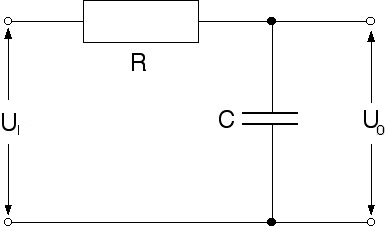
\includegraphics[scale=0.6]{RC_Circuit}
	\caption{1st Order RC Low-Pass Filter}
	\label{fig:1st_Order_RC_Low-Pass_Filter}
\end{figure}
The equation for the output voltage is as follows:
\begin{equation}
U_{\text{O}}=\frac{X_{\text{C}}}{\sqrt{X_{\text{C}}^2+R^2}}\cdot U_{\text{I}}=\frac{1}{\omega\cdot C\cdot\sqrt{\frac{1}{(\omega\cdot C)^2}+R^2}}\cdot U_{\text{I}}=\frac{1}{\sqrt{1+(\omega\cdot C\cdot R)^2}}\cdot U_{\text{I}}
\end{equation}
\\
The following figure \ref{fig:Output_Voltage} shows the measured output voltage values and the fitted curve:
\begin{figure}[H]
	\centering
	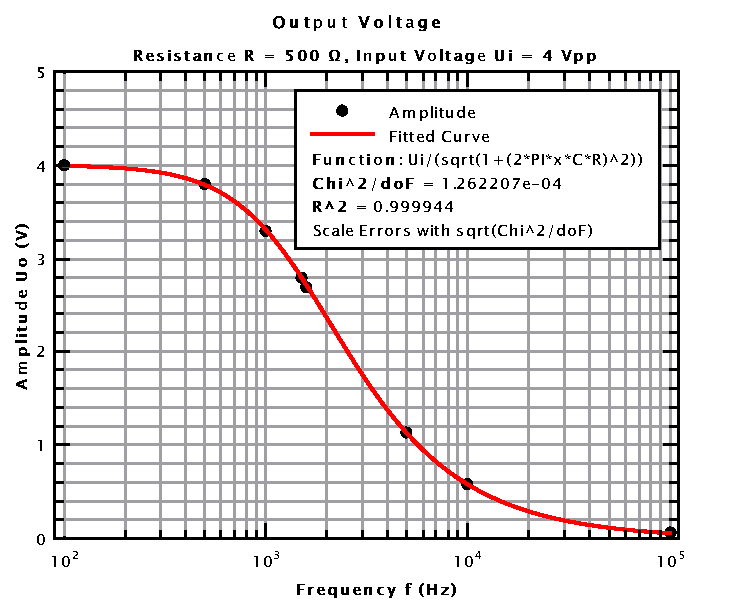
\includegraphics[scale=1]{RC_Low-Pass_Filter_Voltage}
	\caption{Output Voltage}
	\label{fig:Output_Voltage}
\end{figure}
\newpage
The equation for the phase shift is as follows:
\begin{equation}
\varphi=\text{arctan}(-\omega\cdot R\cdot C)
\label{eq:Phase_Shift}
\end{equation}

The phase shift values have been converted from degrees to radians. They can now be plugged directly into the equation \ref{eq:Phase_Shift}.

The following figure \ref{fig:Phase} shows the measured phase shift and the fitted curve:
\begin{figure}[H]
	\centering
	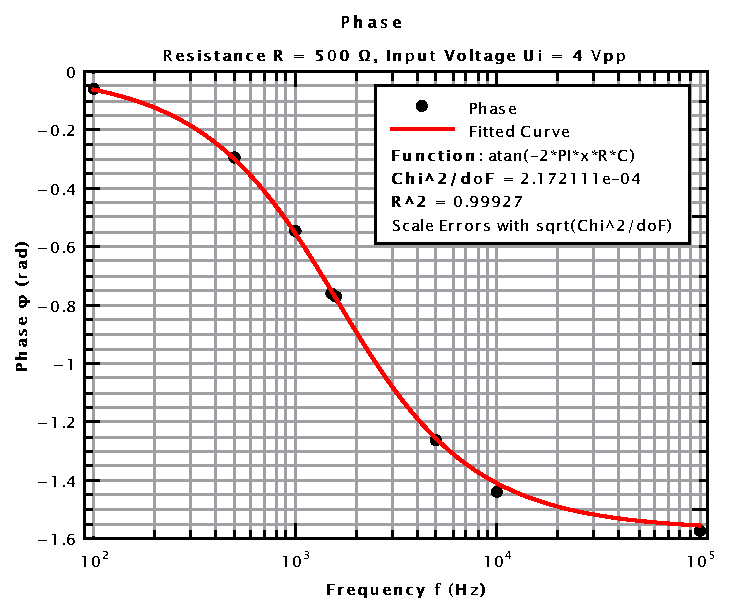
\includegraphics[scale=1]{RC_Low-Pass_Filter_Phase}
	\caption{Phase}
	\label{fig:Phase}
\end{figure}
The values for the Capacity $C$ obtained from QtiPlot are shown in table \ref{tab:Calculated_RC_Calculated_Capacity}:
\begin{table}[H]
	\centering
	\renewcommand{\arraystretch}{1.3}
	\begin{tabular}{r|c}
		& \textbf{Capacity $C$} \\
		\hline\hline
		\textbf{from Output Voltage} & $(216.9\pm0.9)\cdot10^{-9}$\ F \\
		\textbf{from Phase} & $(197.5\pm3.1)\cdot10^{-9}$\ F \\
	\end{tabular}
	\caption{Calculated Capacity}
	\label{tab:Calculated_RC_Calculated_Capacity}
\end{table}
